\chapter{Background}
\label{background}

Information security is a broad topic that covers many different aspects, from which two of them are particularly important for this work: confidentiality and authentication. There are some aspects from cryptography that would be relevant to review, such as asymmetric and symmetric cryptography, as well as the concepts: \emph{plaintext}, \emph{ciphertext}, and \emph{secret key}. In order to explain more advanced topics, number theory and abstract algebra are introduced. Homomorphic encryption is explained thoroughly, noting the mathematical properties and its categories, as well as some possible applications of this type of encryption. The first fully homomorphic encryption scheme is introduced, paving the road for the Brakerski-Gentry-Vaikuntanathan cryptosystem (referred to as the BGV scheme from now on.) Finally, a brief description of cloud computing and its relevant aspects are presented, as well as the impact of secure computation.

\section{Information Security and Data Confidentiality}

Seen from a general perspective, Whitman and Herbert \cite{PrinciplesInformationSecurity} describe security as ``the quality or state of being secure---to be free from danger''. Danger would refer to a potential harming action that an adversary can do, whether it is intentional or not. Computer security is defined by the NIST Computer Security Handbook \cite{NIST95} as follows:
\begin{quotation}
The protection afforded to an automated information system in order to attain the applicable objectives of preserving the \emph{integrity}, \emph{availability}, and \emph{confidentiality} of information system resources (includes hardware, software, firmware, information/data, and telecommunications).
\end{quotation}
This definition introduces two relevant concepts in the previous definition, namely: \emph{information} and \emph{confidentiality}. The RFC 2828 (Request for Comments) publication \cite{shirey2000rfc} defines information as ``facts and ideas, which can be represented (encoded) as various forms of data,'' and data as ``information in a specific physical representation, usually a sequence of symbols that have meaning: especially a representation of information that can be processed or produced by a computer.'' Although both terms have different connotations depending on what they represent, both words are used interchangeably in this work. Now that information has been described as a concept, confidentiality can be introduced. More specifically, data confidentiality refers to the assurance that private or confidential information is not made available or disclosed to unauthorized individuals \cite{CryptoStallings}. This term is closely related to \textit{privacy}, which gives individuals the control of what information related to them may be accessed or stored by whom. Loss of confidentiality would imply unathorized access or disclosure of information.

\section{Cryptography Concepts}

Cryptography is the study of protecting data and communications. It involves communicating messages or information between two or more parties by changing the appearance of the messages, so that it becomes very difficult for unauthorized parties to intercept or interfere with the transmission of the information \cite{IntroCryptoMath}. Cryptography should not be confused with cryptology, because even though they overlap with each other, cryptology includes \emph{cryptanalysis} as well. Without going too deep in the subject, cryptanalysis is defined by Stallings \cite{CryptoStallings}  as the study of principles and methods of transforming an unintelligible message back into an intelligible message \emph{without} knowledge of the secret key. Basically, it studies a cipher to the point where it can be broken, and thus learn the message without having the secret key.

Other important aspects that have been linked to cryptography apart from confidentiality are \textit{authentication} and \textit{integrity}. Authentication gives the receiving parties the means to make sure that the source of the communication is really who it is thought to be, and not someone pretending to be the legitimate sender. On the other hand, integrity, among other things, ensures that the message received has not been tampered in any way. Different kind of cryptographic algorithms are required to satisfy these goals, and the same goes for confidentiality.

Ryabko and Boris \cite{CryptoIT} approach the study of cryptography by explaning the classical problem of transmitting secret messages from a sender A to a receiver B. Both the sender and receiver, A and B, can be thought of persons, organizations, or various technical systems.  They are formally described as abstract ``parties'' or ``entities'', but it is often more convenient to identify both of them as human participants that go by the names of Alice and Bob, instead of using the letters A and B.
For the messages to go from Alice to Bob, there has to be some kind of medium or channel where the information is transmitted. Generally, it is assumed that the channel can be potentially accessed by a third party that is neither the sender nor the receiver. On top of that, it is also assumed that either the receiver or sender has an adversary or enemy E, who is constantly trying to tamper or know the content of the messages passed between Alice and Bob. This attacker E who is constantly eavesdropping on the communication lines is usually called Eve, who is thought to have powerful computing facilities and is able to use methods to learn of the message contents.  It is clear that both Alice and Bob want to protect their messages so that their contents are unclear to Eve. This implies a confidentiality goal, and it can be reached by using encryption algorithms, or as they are commonly known: \emph{ciphers}.

Before a message is sent from Alice to Bob or viceversa, the sender \textit{encrypts} the message. In other words, a certain algorithm is applied on the message so that the content of it is unclear to a third party, such as Eve. Once the sent message has been received by the other party, he \textit{decrypts} it to recover the original content of the message before encryption, known as \textit{plaintext}. In order for this to work, Alice and Bob must have agreed in advance about various of the details needed, such as the algorithm and parameters used by the sender, so that the receiver knows how to perform the decryption properly. Since it would be troublesome that Eve learned of those details, Alice and Bob would have to use some sort of secure channel, such as trusted messengers or couriers, or set up a private meeting where no one else can eavesdrop. Making use of this secure channel, however, is more costly than using the regular communication channel between Alice and Bob, and it might not be available at all times, which is why it is recommended to use it only to agree on some details in advance, like the parameters for the encryption algorithm, as well as a \textit{private key}.

Stanoyevitch \cite{IntroCryptoMath} suggests that the above scheme would make up a cryptosystem, since it makes use of cryptographic algorithms with the purpose of protecting confidentiality. As it has been hinted, such a cryptosystem has two parts: \emph{encryption}, which is done by the sender as means of putting or transforming the actual \textbf{plaintext} into \textbf{ciphertext}, and \emph{decryption}, which is done once the message has been received at the other end and has the purpose of translating the ciphertext back into the original plaintext message. Both encryption and decryption are usually done using a \textbf{key}, and it is intended that only the sender and receiver learn of the nature and value of the key. 

The use of the plaintext, ciphertext, and key concepts are recurrent throughout this work, and given their relevance, they are explained as follows, along with other concepts, the same way Cameron \cite{CryptoNotes} and Stallings \cite{CryptoStallings} describe them.
\begin{description}
\item[Plaintext.-] It is the original message that Alice wants to send to Bob. Neither Bob nor Alice want the message to be known to Eve. This piece of data is fed into the encryption algorithm before it is sent to the other end.
\item[Encryption algorithm.-] This algorithm uses a key that performs several substitutions and transformations on the plaintext. The result is a ciphertext that cannot be translated back to its original plaintext form without the appropriate key.
\item[Secret key.-] It is a value that both Alice and Bob agree upon, it is usually kept secret, since it is used by the encryption algorithm to obtain the ciphertext. The encryption algorithm will produce a distinct output depending on the key being used. In other words, if the secret key is leaked to Eve, this would mean that Eve can now learn any messages that are being produced using that key.
\item[Ciphertext.-] This is the modified or scrambled message produced as output by the encryption algorithm. Its value depends on the algorithm and plaintext, as well as the chosen key.
\item[Decryption algorithm.-] It is like the encryption algorithm, except that its run in reverse. The decryption algorithm has two inputs: the ciphertext and its corresponding key. It then performs the necessary substitutions and transpositions so that the ciphertext is translated back into the original plaintext.
\end{description}

Stinson \cite{stinson2005cryptography} formally defines a cryptosystem as a five-tuple ($\mathcal{P}, \mathcal{C}, \mathcal{K}, \mathcal{E}, \mathcal{D}$), where the following conditions are satisfied:
\begin{enumerate}
\item $\mathcal{P}$ is a finite set of possible plaintexts;
\item $\mathcal{C}$ is a finite set of possible ciphertexts;
\item $\mathcal{K}$, the keyspace, is a set of possible keys;
\item For each $k \in \mathcal{K}$ there is an \textit{encryption rule} $ e_{k} \in \mathcal{E}$  and a corresponding \textit{decryption rule} $ d_{k} \in \mathcal{D}$. Each $e_{k}: \mathcal{P} \rightarrow \mathcal{C}$ and $d_{k}: \mathcal{C} \rightarrow \mathcal{P}$ are functions such that $d_{k}(e_{k}(x))$ for every plaintext element $x \in \mathcal{P}$.
\end{enumerate}

Figure \ref{fig:cryptoflow} depicts the process flow of a simple cryptosystem that is put in place. The plaintext and encryption key is used as input by an encryption algorithm, which results in a ciphertext that gets sent to the other end of the communication line. Then, the ciphertext is used as input by a decryption algorithm, which takes a decryption key H, finally resulting in the original plaintext. Depending on the type of cryptosystem (symmetric or asymmetric), the encryption keys can be considered to be the same or different, i.e.\ $K_{A}\ne K_{B}$ if asymmetric, or $K_{A} = K_{B}$ if symmetric.

\begin{figure}[H]
  \centerline{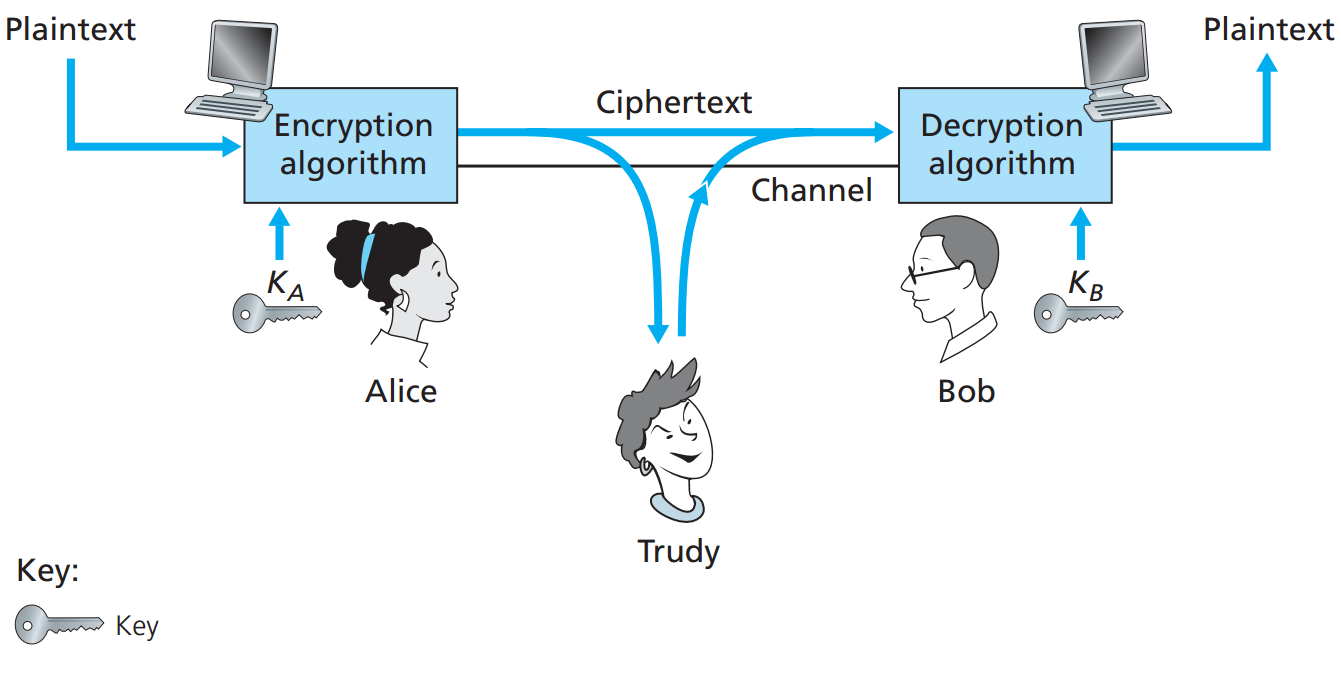
\includegraphics[width=14cm]{img/basic_crypto}}
  \caption[Basic cryptosystem diagram]{Basic cryptosystem diagram. Source: Kurose and Ross \cite{kurose2010computer}.}
  \label{fig:cryptoflow}
\end{figure}


It is assumed at all times that Eve has access to the communication lines, and can always know the ciphertext that is being sent between Alice and Bob. It is also a good practice to assume that the encryption and decryption algorithms are known to Eve, which leaves the key as the most important part of the scheme. As mentioned previously, Alice and Bob need to establish the means to agree on a private key, without anyone else knowing what this key is. As soon as the key is known to the attacker, i.e.\ Eve, all further communication is compromised. When that happens, another key has to be chosen and agreed upon once more by Alice and Bob.

The nature of the encryption and decryption can be classified in two broad categories: symmetric and asymmetric key encryption. Agrawal \cite{CryptoKeys} describes both categories by looking at the keys used. In \textbf{symmetric encryption}, the key used for encryption is virtually the same used in decryption. Therefore, key distribution has to be done before the tranmission of the messages. The key length has a direct impact on the security offered by the encryption algorithm. Meanwhile, \textbf{asymmetric encryption} employs two different keys: public and private. The public key is closely tied to the receiver, and it is used for encryption of the data. It is called public because it is available for general use; therefore, Alice can use Bob's public key to send him messages. On the other hand, the private is kept secret from the outside world, and is only available by an authorized person. The public and private keys always come in pairs, and this is because while the public key is used to encrypt data; its counterpart, the private key, is used to decrypt the data. 

\section{Introduction to Number Theory}

In other to understand more topics pertaining cryptosystems, number theory and its notation, as well as some relevant theorems must be introduced. According to Stark \cite{stark1970introduction}, number theory consists of the study of the properties of whole numbers, and it is considered to be inextricably linked to cryptography. Goodrich \cite{2008algorithm} introduces number theory and most of its relevant aspects, most of which is briefly summarized as follows.

\subsection{Fundamental Theorems}

Given positive integers $a$ and $b$, we use the notation 
\begin{equation}
a|b
\end{equation}
to indicate that $a$ \textbf{divides} $b$, that is, $b$ is a multiple of $a$. If $a|b$, then we know that there is some integer $k$, such that $b=ak$. From this definition, the following properties are found:

\begin{theorem}
  \emph{(Theorem on Divisibility)} Let a, b and c be arbitrary integers,
  \begin{itemize}
  \item If $a|b$ and $b|c$, then $a|c$.
  \item If $a|b$ and $a|c$, then $a|(ib+jc)$, for all integers $i$ and $j$.
  \item If $a|b$ and $b|a$, then $a=b$ or $a= -b$.
  \end{itemize}
\end{theorem}

An integer $p$ is said to be \textbf{prime} if $p\geq 2$ and its only divisors are the trivial divisors $1$ and $p$. Therefore, in the case $p$ is a prime, $p|q$ implies $d=1$ or $d=p$. An integer greater than 2 that is not prime is said to be \textbf{composite}. Also, two integers which only share a common divisor of 1 are considered to be \textbf{relatively prime}.

\begin{theorem}
\emph{(Fundamental Theorem of Arithmetic)}
Let $n > 1$ be an integer. Then there is a unique set of prime numbers $\{p_{1}, \dots p_{k}\}$ and positive integer exponents  $\{e_{1}, \dots , e_{k}\}$, such that
\begin{equation}
n = p_{1}^{e_{1}} \cdots p_{k}^{e_{k}}.
\end{equation}
\end{theorem}

The above product $p_{1}^{e_{1}} \cdots p_{k}^{e_{k}}$ is the prime decomposition of $n$. In other words, any positive integer is made up of the product between two prime numbers.   

\subsection{Modular Arithmetic}

The remainder of $a$ when divided by $n$ is expressed as $a \mod n$, that is:
\begin{equation}
  r = a \Mod{n}.
\end{equation}
\noindent which means that there is some integer $q$, such that
\begin{equation}
  a = qn + r.
\end{equation}

The remainder $r$ is resulting from $a \mod n$ is always an integer in the set $\{0, 1, 2, \dots, n-1\}$, even when $a$ is negative. The integer $n$ is called the \textbf{modulus}. 
\noindent \textbf{Congruence} modulo $n$ is a relevant concept to mention as well. If
\begin{equation}
  a \Mod{n} = b \Mod{n},
\end{equation}
\noindent then we say that $a$ is \textbf{congruent} to $b$ modulo $n$, so it can be written in this way:
\begin{equation}
a \equiv b \Mod{n}.
\end{equation}
Therefore, if $a \equiv b \mod n$, then $a-b=kn$ for some integer $k$. 

Congruences have the following properties:
\begin{equation}
  a \equiv b \Mod{n} \text{ if } n|(a-b)
\end{equation}
\begin{equation}
  a \equiv b \Mod{n} \text{ implies } b \equiv a \Mod{n}
\end{equation}
\begin{equation}
  a \equiv b \Mod{n} \text{ and } b \equiv c \Mod{n} \text{ imply } a \equiv c \Mod {n}
\end{equation}

Suppose that there is a mapping of all integers by the $\pmod n$ operator into the set of integers $\{0, 1, \dots, (n-1)\}$. The technique used to perform arithmetic operations within the confines of this set is known as \textbf{modular arithmetic}. Modular arithmetic exhibits the following properties:
\begin{equation}
  [(a \Mod{n}) + (b \Mod{n})] \Mod{n} = (a + b) \Mod{n}
\end{equation}
\begin{equation}
  [(a \Mod{n}) - (b \Mod{n})] \Mod{n} = (a - b) \Mod{n}
\end{equation}
\begin{equation}
  [(a \Mod{n}) \times (b \Mod{n})] \Mod{n} = (a \times b) \Mod{n}
\end{equation}

And so, the rules for ordinary arithmetic invoving addition, subtraction, and multiplication carry over into modular arithmetic, except that the result is always within the boundaries of the defined set, which is between 0 and $n-1$.

Having explained modulo operation, as well as a having introduced modular arithmetic operations, a very convenient notation, called the set of residues, can be now described. Let $Z_{n}$ denote the set of nonnegative integers less than $n$:
\begin{equation}
Z_{n} = \{0,1,\cdots, (n-1)\}
\end{equation}

The set $Z_{n}$ is also called the set of \textbf{residues}, or \textbf{residue classes} modulo $n$, because if $b=a \mod n$, $b$ is sometimes called the \textbf{residue} of $a$ modulo $n$. The notation $Z_{n}$ represents the integers between 0 and $n-1$. Thus, when it says that ``Let $a$ be a member of $Z_{n}$'', it really means the same thing as ``Let $a$ be an integer between 0 and $n-1$.''

Modular arithmetic in $Z_{n}$, where operations on the elements of $Z_{n}$ are performed mod $n$, show properties similar to those in traditional arithmetic, such as the \textbf{associativity}, \textbf{commutativity}, \textbf{distributivity} of addition and multiplication, and the existence of \textbf{identity} elements 0 and 1 for addition and multiplication, respectively. However, other operations such as division and exponentiation, behave very differently than they do for normal arithmetic. 

Every element $x$ in $Z_{n}$ has an \textbf{additive inverse}, that is, for each $x \in Z_{n}$, there is a $y \in Z_{n}$ such that $x + y \mod n = 0$. In other words, it means there is an element $a'$ that multiplies $a$ modulo $n$ which equals 1.  A \textbf{multiplicative inverse} of $x$ is an element $z^{-1} \in Z_{n}$ such that $xx^{-1} \equiv 1 \mod n$. As well as in regular arithmetic, 0 does not have a multiplicative inverse in $Z_{n}$. There are some nonzero elements that do not have a multiplicative inverse in $Z_{n}$. However, for every $n$ that is prime, every element $x \ne 0$ of $Z_{n}$ has a multiplicative inverse.

\subsection{Order and Generators}

Given a prime $p$ and an integer $a$ between 1 and $p-1$, the \textbf{order} of $a$ is the smallest exponent $e > 1 $ such that
\begin{equation}
  a^{e} \equiv 1 \mod q
\end{equation}

A \textbf{generator}, or primitive root, of $Z_{p}$ is an element $g$ of $Z_{p}$ with order $p-1$. It is called a generator, because the repeated exponentiation of it can generate all the elements in $Z_{p}^{*}$. $Z_{p}^{*}$ is a subset of $Z_{p}$, defined to be the set of integers between 1 and $n$ that are relatively prime to $n$. 

\begin{theorem}
\emph{(Theorem on generators)}
If $p$ is a prime, then set $Z_{p}$ has $\phi(p-1)$ generators.
\end{theorem}

\subsection{Other Relevant Points on Modular Arithmetic}

%\item 
\begin{theorem}
\emph{(Fermat's Little Theorem)}
Let $p$ be a prime, and let $x$ be an integer such that \\ $x \mod p \ne 0$. In other words, that $p$ does not divide the integer $x$. Then
\begin{equation}
x^{p-1} \equiv 1 \pmod{n}
\end{equation}
\end{theorem}

%\item 
\begin{theorem}
\emph{(Euclid's Division Theorem)} For every integer $m$ and positive integer $n$, there exist unique integers $q$ and $r$ such that $m=nq+r$ and $0 \leq r < n$. By definition, $r$ is equal to $m \mod n$.
\end{theorem}

Cliff and Ken \cite{cs21math19notes} review several important concepts regarding modular arithmetic, and are thus listed as follows:

\begin{itemize}
\item \textit{Adding multiples of n does not change values mod n}. That is, \\ $i \mod n= (i+kn) \mod n$ for any integer $k$.

\item Mod (by $n$) can be taken anywhere in calculation, as long as mod $n$ is taken from the final result.

\item \textit{Commutative, associative, and distributive laws}. Addition and multiplication mod $n$ satisfy the commutative and associative laws, and multiplication distributes over addition.

\item The expression ``$x \in Z_{n}$'' is used to mean that $x$ is a variable that can take on any of the integral values between 0 and $n-1$.
\end{itemize}

\section{Abstract Algebra: Groups and Rings}

Stallings \cite{CryptoStallings} describes groups and rings as some of the fundamental elements of a branch of mathematics known as abstract algebra. In abstract algebra, the focus is mostly on those elements that can be operated algebraically; in other words, how two elements of a set can be combined to obtain a third element in the set. The nature of the set is defined by the operations that can be performed on the elements of the set. It has been chosen that, by convention, the two main classes of operations on set elements are usually the same as the notations for addition and multiplication on traditional arithmetic. However, there is not really a limitation on the kind of operations that can be defined using abstract algebra.

\subsection{Groups}

A \textbf{group} G, denoted by $\{ G, \cdot \}$ is a set of elements with a binary operation, which is denoted by the operator $\cdot$. This operator is generic, and can refer not only to multiplication, but also to addition or some other mathematical operation. It associates to each ordered pair $(a, b)$ of elements in G an element $(a \cdot b)$ in G, such that the following axioms are followed:
\begin{description}
  \item[(A1) Closure:] If $a$ and $b$ belong to $G$, then $a \cdot b$ is also in $G$.
  \item[(A2) Associative:] $a \cdot (b \cdot c) = (a \cdot b) \cdot c $ for all $a$, $b$, $c$ in $G$.
  \item[(A3) Identity element:] There is an element $e$ in $G$ such that $a \cdot e = e \cdot a = a$ for all $a$ in $G$.
  \item[(A4) Inverse element:] For each $a$ in $G$ there is an element $a'$ in G such that $a \cdot a' = a' \cdot a = e$. 
\end{description}
It is worth noting that if a group has a finite number of elements, it is called a \textbf{finite group}, and the order of the group is equal to the number of elements in the group. Otherwise, the group is an \textbf{infinite group}. Moreover, a group is said to be \textbf{abelian} if it satifies the following condition, known as the commutative property:
\begin{description}
  \item[(A5) Commutative] $a \cdot b = b \cdot a$ for all $a$, $b$ in $G$.
\end{description}

When the group operation is addition, the identity element is 0; the inverse element of $a$ is $-a$; and subtraction is defined with the following rule: $a-b = a+(-b)$. 
  
\subsection{Rings}

A \emph{ring} $R$, which is sometimes denoted by $\{R, +, \times \}$, is a set of elements with two binary operations, called \textit{addition} and \textit{multiplication}, such that for all $a$, $b$, $c$ in $R$, there are some axioms that must be obeyed. It must be pointed out that a ring fulfills the same axioms as an abelian group with respect to addition; that is, axioms A1 through A5. The rest of the axioms obeyed by a ring are listed as follows:
\begin{description}
\item[(M1) Closure under multiplication:] If $a$ and $b$ belong to $R$, then $a \times b$ is also in $R$.
\item[(M2) Associativity of multiplication:] $a(b \times c) = (a \times b)c$ for all $a$, $b$, $c \in R$.
\item[(M3) Distributive laws:] $a(b+c) = (a \times b) + (a \times c)$ for all $a$, $b$, $c$ in $R$. \\ $(a+b)c = (a \times c) + (b \times c)$ for all $a$, $b$, $c$ in $R$.
\end{description}

Essentially, a ring is a set in which addition, subtraction $[a-b = a + (-b)]$, and multiplication can be done without leaving the set. Furthermore, a ring is said to be \textbf{commutative} if it satisfies the following additional condition:
\begin{description}
\item[(M4) Commutativity of multiplication:] $(a \times b) = (b \times a)$ for all $a$, $b$ in $R$.
\end{description}

Additionally, there are other axioms that, if obeyed, turn the commutative ring into an \textbf{integral domain}. These axioms are:  
\begin{description}
\item[(M5) Multiplicative identity:] There is an element 1 in $R$ such that \\ $(a \times 1) = (1 \times a) = a$ for all $a$ in $R$.
\item[(M6) No zero divisors:] If $a$, $b$ in $R$ and $(a \times b)=0$, then either $a=0$ or $b=0$.
\end{description}

\subsection{Homomorphisms}

As it has been previously noted, operations within a closed group always result in another element from the group. Only one operation is allowed in a group: addition or multiplication, for instance. There may also be two groups or sets that are made up of different elements, each with its own operation. A \emph{homomorphism} consists of the construction of a function that \emph{translates} elements from one group to another group with the same properties.

\subsubsection{Group Homomorphism}

According to Beachy and Blair \cite{beachy2006abstract}, a homomorphism is defined as follows: Let $G_{1}$ and $G_{2}$ be groups, and let $\phi: G_{1} \rightarrow G_{2}$ be a function. Then $\phi$ is said to be a \textbf{group homomorphism} if
\begin{equation}
\phi(a*b) = \phi(a) *' \phi(b)
\end{equation}
for all $a$, $b$ in $G_{1}$.

Consider the example presented by Sorzano \cite{sorzano2013}, where there are two sets: $S= \{a, b, c\}$ and $S' = \{A, B, C\}$  with the operations $*: S \times S \rightarrow S$ and $*' : S' \times S' \rightarrow S'$. The operations within each group map two elements to another element from the same group. For example, $b*c=a$ and $a*a=a$, and in the other group, $A*A = A$ and $B*C=A$. So it can be seen that there is some similarity in the nature of the operations from both groups. Now consider the homomorphism between both groups, where:
\[
\begin{split}
  \phi: S \rightarrow S' \\
  \phi(a) = A \\
  \phi(b) = B \\
  \phi(c) = C \\
\end{split}
\]

\noindent Therefore, the following holds true using the above homomorphism:

\begin{equation}
b*c=a \rightarrow \phi(b) *' \phi(c) = \phi(a) \rightarrow B *' C = A
\end{equation}

What this means is that a homomorphism serves as a link to translate operations from one group to the other, keeping the same properties.

\subsubsection{Ring Homomorphism}

Similarly to groups, there are also homomorphisms for rings, the main difference being that, instead of a single operation, two operations are considered.

Let $R$ and $S$ be rings with addition and multiplication. The map $\phi: R \rightarrow S$ is a homomorphism if:
\begin{enumerate}
\item $\phi$ is a group homomorphism on the additive groups $(R, +)$ and $(S,+)$
\item $\phi(xy) = \phi(x) \phi(y)$ $\forall x, y \in R$
\end{enumerate}

\section{Homomorphic Encryption}

Homomorphic is a word that has its roots in Greek, and it means ``the same shape''. It is used in various areas, such as abstract algebra, which then inspired its use in cryptography. This concept refers to the ability to make computations, i.e.\ operations such as addition and multiplication, on encrypted data without sharing the secret key to decrypt the data prior to the computations. 

Before homomorphic encryption, any change to the secret value contained in a ciphertext required the corresponding secret key, so that it could be decrypted, applied the change, and re-encrypted. However, homomorphic encryption eliminates the need of sharing the secret key, especially with those that are not to be completely trusted, in the event that there is some change that must be applied to encrypted data. 
Lange \cite{lange2011} mentions several applications that would benefit from a homomorphic encryption function, given its ability to manipulate encrypted data. Such applications fall in the domain of: e-cash, e-voting, private information retrieval (encrypted databases), and cloud computing.

%\subsection{What is Homomorphic Encryption?}
According to P{\"o}tzelsberger \cite{potzelsberger2013kv}, when the encryption function of a cryptosystem is a homomorphism, meaning that it preserves group operations performed on ciphertexts, it is called a \emph{homomorphic cryptosystem}. The group operation considered for this kind of cryptosystem is either the arithmetic addition or multiplication, or both. A homomorphic encryption is additive if:
\begin{equation}
\mathcal{E}(x+y) = \mathcal{E}(x)\otimes \mathcal{E}(y)
\end{equation}

where $\mathcal{E}$ denotes an encryption function, $\otimes$ denotes an operation depending on the used cipher and $x$ and $y$ are plaintext messages. A homomorphic encryption is multiplicative if:
\begin{equation}
\mathcal{E}(x \cdot y) = \mathcal{E}(x) \otimes \mathcal{E}(y)
\end{equation}

where again $\mathcal{E}$ denotes an encryption function, $\otimes$ denotes an operation depending on the used cipher and $x$ and $y$ are plaintext messages.

The above conditions denote that the result of the operations between both inputs, in this case $x$ and $y$, is going to be the same whether the operations are performed after or before encryption. This property is what makes it possible to perform computations on an encrypted value which later can be decrypted to the correct result.

\subsection{Classification of Homomorphic Encryption Schemes}

Homomorphic encryption schemes are classified in two broad groups, depending on how they are defined, namely: partially homomorphic and fully homomorphic. 

\emph{Partially homomorphic encryption} schemes are defined over a group, and they support one operation at most: either addition or multiplication. On the other hand, \emph{fully homomorphic encryption} schemes are defined over a ring, and can support up to two operations: addition and multiplication.

According to P{\"o}tzelsberger \cite{potzelsberger2013kv}, even though somewhat homomorphic cryptosystems support a limited number of homomorphic operations, they are the building blocks for fully homomorphic encryption, and provide much more efficiency and shorter ciphertexts than their fully homomorphic counterparts. 


\subsection{Explaining Homomorphic Encryption}

Craig Gentry \cite{homoenc} explains the concept behind homomorphic encryption in a very simple way. Imagine that Alice has a jewelry store and wants her workers to assemble raw materials (diamonds, gold, silver, etc.) into finished products (necklaces, rings, etc.), but does not trust them, thinking they might run off with the raw materials at their first chance. So instead of giving them direct access to the materials, Alice places the materials inside a transparent glove boxes, which are then promptly locked with a key that only Alice has. This way, workers can put their hands inside the gloves that are connected to the box, and through them, work with the raw materials. Additionally, the workers are able to put in things inside the boxes, such as soldering iron to use on the raw materials, even though they cannot take anything out of it, since they do not have the key to open the box. Once the products are finished, Alice can then recover the products from the box using her key. The analogy is not perfect, because the workers are able to see the materials while working on them, but it is relevant because homomorphic encrytion means that they cannot take the materials with them.

Hayes \cite{Hayes2012} offers a proof of concept that accurately describes the very essence of a homomorphic cryptosystem. It is shown as follows: consider that the plaintext consists of integers; to encrypt a number, double it; to decrypt it, divide by 2. Using this scheme, addition and a nonstandard version of multiplication can be done on the encrypted data. Given the plaintext inputs $x$ and $y$, we can encrypt each of them separately, add the ciphertexts, and finally decrypt the result. This calculation would give the correct answer, expressed as $2x+2y=2(x+y)$. In other words, it is the same result as if each plaintext input were multiplied separately and then added with each other, because in the end, dividing it by two causes the same effect on both sides. 
Regarding multiplication, a little tweak has to be done for it to work. The product of the ciphertexts is defined as $(\frac{1}{2}) C_x C_y$, while the plaintexts are multiplied by the regular formula $xy$. 
As an example, consider $x=5$ and $y=7$. The result of the multiplication would come as $x \times y = 35$. To perform the same evaluation between ciphertexts, both inputs would be encrypted following the rule previously defined:
\begin{equation}
C_{x} = 5 \times 2 = 10
\end{equation}
\begin{equation}
C_{y} = 7 \times 2 = 14
\end{equation}
The multiplication is performed as $(\frac{1}{2}) 10 \times 14 = 70$, and it is divided by 2 to decrypt the ciphertext: $\frac{70}{2} = 35$, which turns out to be the correct result of the multiplication.

Certainly, the above cryptosystem is considered to be \emph{fully homomorphic}, since it supports both addition and multiplication. However, it is definitely not a secure one, since anyone that knows of the workings of the cipher can easily get to learn the secret message. This is also partly the reason of why the encryption and decryption algorithms are not usually kept as a secret, because it would be quite impractical to make a different encryption and decryption algorithm every time it were discovered. 

Stuntz \cite{stuntz2010} provides an example of a cipher scheme that has an inherent homomorphic property. Consider the popular, yet unsecure, ROT13 cipher, also known as the Caesar cipher. The ROT13 is a simple substitution cipher which changes each letter with the letter that is thirteen positions ahead on encryption. To do decryption, it does the opposite: each character goes back thirteen positions in the alphabet. 
ROT13 is partially homomorphic with respect to the concatenation operation, because it is possible to concatenate two different pieces of ciphertexts. At decryption, the concatenation of the two pieces of ciphertexts ends up to be same as the concatenation of the original messages, the plaintext. Therefore, it is partially homomorphic with respect to concatenation. 

Consider, for instance, the plaintext pair $P_{1}=$ HELLO and $P_{2}=$ WORLD, which both concatenate to ``HELLOWORLD''. If both plaintexts were encrypted using ROT13, the ciphertexts would be $C_{1}=$ URYYB and $C_{2}=$ JBEYQ, and if concatenated, ``URYYBJBEYQ''. Therefore, if the result of the ciphertext concatenation were decrypted, it would result in ``HELLOWORLD'', which is exactly the same message obtained when the pair of plaintexts were concatenated originally. Figure \ref{fig:homosample} shows the aforementioned example as it goes through the encryption and decryption processes. 

\begin{figure}[H]
  \centerline{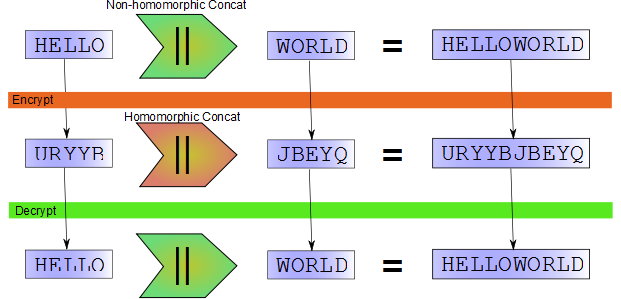
\includegraphics[scale=0.5]{img/rot13homo}}
  \caption[Example of the homomorphic property in ROT13]{Example of the homomorphic property in ROT13. Source: Stuntz \cite{stuntz2010}.}
  \label{fig:homosample}
\end{figure}

\subsection{The First Fully Homomorphic Encryption Scheme}

In an article published by the research staff of the NSA \cite{NSA2014}, it is discussed how the term of fully homomorphic encryption has been around for about 30 years, and only recently, in 2009 to be exact, a very important breakthrough regarding fully homomorphic encryption was made by Craig Gentry. Thanks to this breakthrough, the first fullly homomorphic scheme was created, opening the doors of research to this topic that was thought to be at a dead end. 

As Gentry \cite{homoenc} himself points out, by ``fully'' it means that there are no limitations on what manipulations can be performed on the ciphertext. Given ciphertexts $c_{1}, \dots, c_{t}$ that encrypt $m_{1}, \dots, m_{t}$ with a fully homomorphic encryption scheme under some key, and given any efficiently computable function $f$, anyone can efficiently compute a ciphertext (or set of ciphertexts) that encrypts $f(m_{1}, \dots, m_{t})$ under that key. This permits all kinds of computations on the encrypted data. Of course, no information about the plaintexts $m_{1}, \dots, m_{t}$ or the value of $f(m_{1}, \dots, m_{t})$ is leaked. 

The first step in Gentry's blueprint was to construct a \emph{somewhat homomorphic encryption scheme} (SWHE), which was capable of evaluating ``low-degree'' polynomials homomorphically. In order to obtain a fully homomorphic encryption scheme, Gentry proposed a \emph{bootstrapping theorem} which made it possible to transform the original somewhat homomorphic encryption scheme into a \emph{leveled} fully homomorphic encryption one.

One of the main problems that fully homomorphic encryption faces is the managing of ``noise'' in the ciphertext. In this case, noise refers to the gradual distortion of ciphertexts that is caused by doing operations (e.g., addition or multiplication) on them. As more operations are performed on the ciphertext, the larger the noise becomes, rendering the ciphertext undecipherable, as it would end up with the wrong result after attempting to decrypt. As Hayes \cite{Hayes2012} points out, each homomorphic addition doubles the noise, and each multiplication squares it. Thus, the number of operations must be limited, should one not wish to ``corrupt'' the ciphertext. 

An obvious solution to the problem of accumulating noise is to decrypt the data and re-encrypt it whenever the noise begins to approach the critical threshold. Thus, the noise is resetted to its original level, allowing for more operations. The problem with this approach is that decryption needs the secret key, which is usually not going to be available to whoever is performing the operations on the ciphertext. 

Instead, Gentry developed a process called \emph{bootstrapping} to overcome the problem of noise accumulation. The \emph{evaluate} function used in the cryptosystem can virtually perform any computation, as long as it has not reached the critical threshold of noise. Therefore, that very function is used to run the \emph{decrypt} function, which takes as input the noise-heavy ciphertext that has gone through several operations, and the \emph{encrypted secret key}. This makes sense because the decrypt function relies on the evaluate function, which was made to work on encrypted values. So when the \emph{decrypt} function is run, the decrypted result is not the plaintext, but rather a new encryption, with reduced noise. This process of re-encrypting and refreshing the noisy ciphertext can be repeated as many times as needed, because then it technically has no limitations on the number of operations it can perform. However, extra layer of encryption will consequently increase the overall computational effort required to complete the set of operations desired to be performed. As the research staff from the NSA exemplifies \cite{NSA2014}, if the process were to be used by Google to search the web homomorphically, the normal computing time required would be multiplied by about a trillion. This is the reason why this scheme is not practical enough as a solution for implementation.

\subsection{Learning with Error Problems}

Some problems are considered \emph{hard} to solve, meaning that no polynomial time algorithm is known. However, this is a good thing in cryptography, since data encryption relies on the computational difficulty to solve problems. As the slides by Sahni \cite{sahni1999} point out, many modern cryptosystems rely on the difficulty of these problems, such as RSA and Elliptic Curve Cryptography.

Blum \cite{Blum:1993:CPB:646758.759585} suggests that learning problems have certain properties which make them possible sources of cryptographic hardness. Two of these problems are the learning with errors problem, and its variation, the ring-learning with error problem.

The learning with errors (LWE) problem was introduced by Regev \cite{Regev:2005:LLE:1060590.1060603}; it is defined as follows:

\theoremstyle{definition}
\begin{definition}
{Learning with Errors Problem}
For security parameter $\lambda$, let $n = n(\lambda)$ be an integer dimension, let $q=q(\lambda) \geq 2$ be an integer, and let $\chi = \chi(\lambda)$ be a distribution over $\mathbb{Z}$. The LWE $(n, q, \chi)$ problem is to distinguish the following two distributions: In the first distribution, one samples $(a_{i},b_{i})$ uniformly from $\mathbb{Z}_{q}^{n+1}$. In the second distribution, one first draws $s \leftarrow \mathbb{Z}_{q}^{n}$ uniformly and then samples $(a_{i}, b_{i}) \in \mathbb{Z}_{q}^{n+1}$ by sampling $a_{i} \leftarrow \mathbb{Z}_{q}^{n}$ uniformly, $e_{i} \leftarrow \chi$, and setting $b_{i} = \left \langle a,s  \right \rangle + e_{i}$. The LWE $(n, q, \chi)$ assumption is that the LWE $(n, q, \chi)$ problem is infeasible.
\end{definition}

Regev proved that for certain moduli $q$ and Gaussian error distributions $\chi$, the LWE $(n, q, \chi)$ assumption is true as long as certain worst-case lattice problems are hard to solve using a quantum algorithm. Later, Peikert \cite{Peikert:2009:PCW:1536414.1536461} de-quantized Regev's results, proving that the LWE $(n, q, \chi)$ assumption is true as long as certain worst-case lattice problems are hard to solve using a \emph{classical algorithm} as well.

At a later date, the ring learning with errors (RLWE) problem was introduced by Lyubaskevsky et al. \cite{rlwe2010}. The learning with errors (LWE) problem and the ring learning with errors (RLWE) problem are syntactically identical, aside from using different rings (the first one uses $\mathbb{Z}$ and the second one a polynomial ring). 

Regev \cite{regevlearning} gives a convenient definition of the ring-LWE problem. Let $n$ be a power of two, and let $q$ be a prime modulus satisfying $q=1 \mod 2n$. Define $R_{q}$ as the ring $\mathbb{Z}_{q}[X] / \left \langle x^{n} + 1 \right \rangle$ containing all polynomials over the field $\mathbb{Z}_{q}$ in which $x^{n}$ is identified with $-1$. In ring-LWE, we are given samples of the form $(a, b = a \cdot s + e) \in R_{q} \times R_{q}$, where $s \in R_{q}$ is a fixed secret, $a \in R_{q}$ is chosen uniformly, and $e$ is an error term chosen independently from some error distribution over $R_{q}$. The goal is to recover the secret $s$ from these samples (for all $s$, with high probability).

Because of the hardness and versatibility of both problems, they have become popular as the basis for cryptographic constructions. Regev \cite{regevlearning} notes that LWE has been used as the basis of public-key encryption schemes that are considered secure under chosen-plaintext attacks, chosen ciphertext attacks, oblivious transfer protocols, and more.

To understand how a LWE can be applied in cryptography, consider the following simple cryptosystem described by Regev \cite{regevlearning}, which is parameterized by integers $n$ (the security parameter), $m$ (number of equations), $q$ (modulus), and a real $\alpha > 0$ (noise parameter). One possible choice that guarantees both security and correctness is the following. Choose $q$ to be a prime between $n^2$ and $2n^2$, $m=1.1 \cdot n\log q$, and $\alpha = \dfrac{1}{\sqrt{n} \log^{2}n}$. All additions are performed modulo $q$ in the following description. 

\begin{itemize}
\item \textbf{Private key}: The private key is a vector $s$ chosen uniformly from $\mathbb{Z}_{q}^{n}$.
\item \textbf{Public key}: The public key consists of $m$ samples $(a_{i}, b_{i})_{i=1}^m$ from LWE distribution with secret $s$, modulus $q$, and error parameter $\alpha$.
\item \textbf{Encryption}: For each bit of the message, choose a random set $S$ uniformly among all $2^m$ subsets of $[m]$. The encryption is $(\sum_{i \in S} a_{i}, \sum_{i \in S} b_{i})$ if the bit is 0 and $(\sum_{i \in S} a_{i}, \left \lfloor{\frac{q}{2}}\right \rfloor + \sum_{i \in S} b_{i})$ if the bit is 1.
\item \textbf{Decryption}: The decryption of a pair $(a,b)$ is 0 if $b - \left \langle a,s \right \rangle$ is closer 0 than to $\left \lfloor \frac{q}{2} \right \rfloor$ modulo $q$, and 1 otherwise. 
\end{itemize}
Such a cryptosystem is quite inefficient, but it serves its purpose to establish a link between the LWE problem and its use in cryptography.

Hayes \cite{Hayes2012} writes in his article that recently, Brakerski, Vaikuntanathan and Gentry have developed a variant of the learning-with-errors system that takes a different approach to noise management. Instead of stopping the computation at intervals to re-encrypt the data, they incrementally adjust parameters of the system after every computational step in a way that prevents the noise level from ever approaching the limit.

\subsection{Brakerski-Gentry-Vaikuntanathan Scheme}

The Brakerski-Gentry-Vaikuntanathan (BGV) scheme \cite{cryptoeprint:2011:277} is a leveled fully homomorphic encryption that does not rely on bootstrapping, but rather employs it as an optimization. However, it still follows Gentry's blueprint to build a fully homomorphic cryptosystem, thus lattice-based cryptography is employed, albeit with certain improvements. It is described as \emph{leveled} in the sense that the parameters of the scheme depend (polynomially) on the depth of the circuits that the scheme is capable of evaluating.

This scheme dramatically improves performance compared to previous attempts at fully homomorphic encryption, and also bases security on weaker assumptions. The security of the BGV scheme is based on the ring-learning with error (RLWE) problem that has a $2^{\lambda}$ security against known attacks.

As it happens with the first fully homomorphic encryption scheme proposed by Gentry \cite{homoenc}, making computations on the ciphertext creates a noise that gradually accumulates. Specifically, performing one addition between two ciphertexts roughly doubles the noise, while multiplication squares it. Decryption succeeds as long as the magnitude of the noise does not surpass a certain threshold. However, the BGV scheme proposes a \emph{noise-management technique} that keeps the noise in check by reducing  it after doing homomorphic operations, without depending on the bootstrapping technique previously mentioned. The noise management technique is called \emph{modulus switching}, and it was developed by Brakerski and Vaikuntanathan \cite{cryptoeprint:2011:344}, albeit with a modification. 

The lemma that describes the original modulus-switching technique says that an evaluator who does not know the secret key $s$, but instead only knows a bound on its length, can transform a ciphertext $c$ modulo $q$ into a different ciphertext modulo $p$ while preserving correctness. This is expressed as $[\left \langle c',s \right \rangle]_{p} = [\left \langle c,s  \right \rangle]_{q} \mod 2$. The interesting property found here is that if $s$ is short and $p$ is sufficiently smaller than $q$, then the ``noise'' in the ciphertext actually decreases, meaning that $|[\left \langle c',s \right \rangle]_{p}| < |[\left \langle c,s \right \rangle]_{q}|$. This technique allows the evaluator to reduce the magnitude of the noise without knowing the secret key, and without depending on bootstrapping. The BGV scheme takes the aforementioned technique, and further improves noise management by making use of a \emph{ladder of gradually decreasing moduli}.  

This homomorphic scheme has been implemented as a software library in C++, called HElib \cite{helib}. The implementation focuses on the effective use of the Smart-Vercauteren ciphertext packing techniques and the Gentry-Halevi-Smart optimizations. Halevi and Shoup \cite{cryptoeprint:2014:106} describe in a paper the algorithms employed on the implementation, as well as some considerations to have in mind depending on the hardware used.

\subsection{Applications}

As it was previously mentioned, various individuals and corporations are hesitant to make use of cloud services, mainly because of the security risks it poses, such as privacy loss and tampering of the data. Traditional cryptosystems can protect confidentiality if the only goal is remote storage; but it is restricted to just that. However, if the encryption employed were homomorphic, the cloud server where the data is stored would be able to perform meaningful computations on the encrypted data.  The scenarios where homomorphic encryption can be applied are many, and some of the most important areas are: medical applications, financial applications, advertising and pricing, electronic voting, data mining, and biometric authentication.

\begin{description}
\item[Medical applications.-] A straightforward application of homomorphic encryption in a medical context is the storage and processing of medical records of patients. Most of the time, these records are considered private, but a hospital would be greatly benefited if it could rely on a cloud service rather than setting up its own data center. If homomorphic encryption has been used as a cipher to protect the medical records, then there could be meaningful pieces of information that could be extracted from it. For example, if a doctor in another clinic was granted access to the patient's medical record, he could make use of a function that makes homomorphic evaluations on the encrypted record to obtain statistical data from the patient. And this would be possible without the cloud server learning what information the medical record contained.
\item[Financial applications.-] Data about corporations, such as their stock price, performance or inventory is often considered to be private, and also very relevant towards making investment decisions. There are many kinds of computations that could be done on this private data, such as running predictive simulations on stock price performance. 
\item[Advertising and pricing.-] Nowadaways, user activity is heavily monitored by the websites that he browses, and uses this data as to build a profile and direct to him appropriate ads. Take Amazon as an example: Amazon keeps a history on what items the user is looking at, even if they were not bought, for further advertising. The user might get emails advertising the same or similar products, or might even see the same ads on unrelated sites, such as Facebook \cite{KimMai}. 
  The above example is just the tip of the iceberg. There is a lot of contextual information that can be retrieved from the user to gain insight on his interests and current status, without him having to be active. For example, he could be suscribed to a service that sends alerts to his smartphone whenever he is walking nearby a shop that could be of his interest. Geolocation and user profile are pieces of information that are considered to be private, the user might not subscribe to the service if it just shared around his information. If, however, he is guaranteed that his information is being kept encrypted, and that it stays that way whenever a computation is made to see if there is a nearby store of his interest, then he might not be as reluctant to make use of the service. The applications on advertising using homomorphic encryption are diverse, because there are pieces of data that can be obtained passively, such as the user's geolocation or browsing habits.
\item[Electronic Voting.-] Although not necessarily related to cloud computing, electronic voting is another area where homomorphic encryption can make such voting scheme feasible and convenient. Voting could be done from anywhere as long as the participant is provided with Internet access. Simply put, homomorphic encryption can be used to hide the content of a ballot by calculating the total number of votes, without having to decrypt any of the ballots. However, electronic voting is not as trivial as it seems, because apart of confidentiality, there are other security parameters that are equally important, such as: correctness of the tally, democracy, robustness, verifiability, fairness, and verifiable participation. Therefore, applying homomorphic encryption would only satisfy one of the many requirements for electronic voting to be feasible.
\item[Data mining.-] Closely related to advertisement, data mining has several issues on privacy. Using homomorphic encryption would mean that certain sensitive attributes of customers data can be protected from unauthorized parties. Yang et al. \cite{YangZhongWright} have proposed a solution that allows a data miner to compute frequencies of values or tuples of values in the customers' data in a privacy preserving manner. The advantage of this solution is that, unlike other existing attempts to make data mining more private, is that this solution is both fully private and fully accurate, without compromising one in exchange of the other.
\item[Biometric Authentication.-] Biometric authentication is an area of application quite different from the rest. This is because biometric data is assumed to be public, since fingerprints virtually on every object touched by a person. Therefore, according to P{\"o}tzelsberger \cite{potzelsberger2013kv}, what is considered to be private is the relationship between the biometric data and the person from whom it comes. It can be applied on the scenario where the user tries to authenticate using one of his biometric features: the biometric feature would be stored and encrypted before it looks for a match in the database. The homomorphic evaluation would consist in the comparison between the user's biometric feature and all of the existing rows in the database. Traditional cryptographic would not be appropriate for this task, since biometric data can vary slightly each time, so an exact match would not work out. Assuming that the biometric feature is stored as a binary string, the homomorphic evaluation would consist in computing the Hamming distance between two feature vectors, and a predefined threshold to achieve the comparison. This is how the biometric data itself can stay public, but the relationship of whom it belongs to is kept private.
\end{description}

\section{Services in the Cloud}

The cloud, a trendy term used to describe a network of servers usually accessible through the Internet, currently provides two important services: storage and computation. As Xu et al. in \cite{cryptoeprint:2011:574} point out, cloud storage services, such as Dropbox, Skydrive, Google Drive, and Amazon S3 have become very popular in recent years. As the use of these services become more common, more sensitive information is kept in the cloud, such as emails, health records, private videos and photos, company finance data, government documents, etc. 

Li et al. \cite{cryptoeprint:2009:593} introduce cloud computing as a new term that views computing as a utility which enables convenient, on-demand access to computing resources that can be rapidly deployed with minimal management overhead and great efficiency. Cloud computing has the potential to benefit its users in avoiding large capital expenditure used for deployment and management of both software and hardware, such as setting up a data center. 

All of these services are opening up a new era powered by the software as a service (SaaS) computing architecture. One of the main advantages of storing this information in the cloud is that the owners are relieved from the burden of data storage and maintenance at all times. There are many plans that adjust to the on-demand needs of the owner of the data, which is way less costly than building and maintaining a whole data center. This implies that the clients of these services can expect to gain reliability and availability from having the data stored remotely. On the other hand, the data is necessarily brought out of their control and protection. This becomes a risk for the owner of the data, since the information stored in the cloud could potentially be accessed by unauthorized individuals, such as competitors or malicious attackers. There also exists the possibility that the information stored could be tampered in some way, thus compromising its integrity. Therefore, the computing and storage service providers are usually not trusted completely, which is why it has been difficult for the public and organizations to fully adopt the use of these services.

The aforementioned issue brings up the need of having a mechanism that verifies that a cloud provider is storing the whole database intact, even the portions that are rarely accessed. Ateniese et al. \cite{cryptoeprint:2014:886} point out that, fortunately, a series of \textit{proofs-of-storage} protocols have been proposed to solve this problem related to data integrity. Xu et al. \cite{cryptoeprint:2014:395} define a proof of storage (POR or PDP) as a cryptographic tool, which enables a data owner or third party auditor to audit integrity of data stored remotely in a cloud storage server, without keeping a local copy of data or downloading data back during auditing. In other words, applying a proof of storage in a cloud server can guarantee that the data has not been tampered with; and in the event that it is, most likely the service could be held liable for damages to the data. A huge advantage of using a proof of storage is that the data does not have to be downloaded to confirm its integrity, which makes it ideal to make use of it routinely. 

One of the simplest use cases for cloud computing is when a user independent from the cloud wants to store some data in it for later retrieval. In this simple case, data confidentiality and integrity can be trivially ensured. For that, typical cryptography primitives can be used by encrypting the user's data before it is sent for storage in the cloud. To ensure confidentiality, the key used for encryption is kept secret from the cloud provider. However, real life applications are not as simple. Damgard et al. \cite{cryptoeprint:2013:629} mentions that the cloud is more than a storage medium; in particular, computation over the stored data is outsourced to the cloud. Sometimes it might even be distributed among distinct cloud servers geographically apart, operated by different parties. Wang et al. \cite{cryptoeprint:2009:081} describe the nature of the problem at length, because usually a cloud service is not solely restricted as a data warehouse. The data stored in the cloud may be frequently updated by the users, including insertion, deletion, modification, appending, reordering, etc. This kind of complex scenario is what makes the use of traditional cryptographic primitives so difficult to adapt, especially because the data is not stored in a single cloud server, but is instead redundantly stored in multiple physical locations to further reduce the data integrity threats. Therefore, making use of cloud services highly improve data avalability and storage flexibility, data confidentiality and integrity is put at risk.

In order to tackle these issues, there have been many attempts to make cloud services, especially cloud computing, more secure. These attempts are very different in nature, though very similar regarding its goals. These are \textit{secure multi-party computation} and \textit{homomorphic encryption}. David, Nishimaki, et al. \cite{cryptoeprint:2015:135} describes secure multiparty computation (MPC) as the means to allow mutually distrustful parties to compute functions on private data that they hold, without revealing data to each other. There are many methods and approaches proposed to perform secure multiparty computation, although only recent attempts are considered to be efficient enough for application. On the other hand, homomorphic encryption is based on the idea of performing computations on the ciphertext that has gone through an encryption algorithm, without having to decrypt it beforehand. This aspect makes homomorphic encryption a good technique for cloud services, since only the authorized users are able to decrypt the ciphertext after the necessary computations have been performed on it.

%Pendiente hacer un resumen del capitulo y ligarlo al siguiente capitulo

\clearpage
